\documentclass{article}\usepackage[]{graphicx}\usepackage[]{xcolor}
% maxwidth is the original width if it is less than linewidth
% otherwise use linewidth (to make sure the graphics do not exceed the margin)
\makeatletter
\def\maxwidth{ %
  \ifdim\Gin@nat@width>\linewidth
    \linewidth
  \else
    \Gin@nat@width
  \fi
}
\makeatother

\definecolor{fgcolor}{rgb}{0.345, 0.345, 0.345}
\newcommand{\hlnum}[1]{\textcolor[rgb]{0.686,0.059,0.569}{#1}}%
\newcommand{\hlstr}[1]{\textcolor[rgb]{0.192,0.494,0.8}{#1}}%
\newcommand{\hlcom}[1]{\textcolor[rgb]{0.678,0.584,0.686}{\textit{#1}}}%
\newcommand{\hlopt}[1]{\textcolor[rgb]{0,0,0}{#1}}%
\newcommand{\hlstd}[1]{\textcolor[rgb]{0.345,0.345,0.345}{#1}}%
\newcommand{\hlkwa}[1]{\textcolor[rgb]{0.161,0.373,0.58}{\textbf{#1}}}%
\newcommand{\hlkwb}[1]{\textcolor[rgb]{0.69,0.353,0.396}{#1}}%
\newcommand{\hlkwc}[1]{\textcolor[rgb]{0.333,0.667,0.333}{#1}}%
\newcommand{\hlkwd}[1]{\textcolor[rgb]{0.737,0.353,0.396}{\textbf{#1}}}%
\let\hlipl\hlkwb

\usepackage{framed}
\makeatletter
\newenvironment{kframe}{%
 \def\at@end@of@kframe{}%
 \ifinner\ifhmode%
  \def\at@end@of@kframe{\end{minipage}}%
  \begin{minipage}{\columnwidth}%
 \fi\fi%
 \def\FrameCommand##1{\hskip\@totalleftmargin \hskip-\fboxsep
 \colorbox{shadecolor}{##1}\hskip-\fboxsep
     % There is no \\@totalrightmargin, so:
     \hskip-\linewidth \hskip-\@totalleftmargin \hskip\columnwidth}%
 \MakeFramed {\advance\hsize-\width
   \@totalleftmargin\z@ \linewidth\hsize
   \@setminipage}}%
 {\par\unskip\endMakeFramed%
 \at@end@of@kframe}
\makeatother

\definecolor{shadecolor}{rgb}{.97, .97, .97}
\definecolor{messagecolor}{rgb}{0, 0, 0}
\definecolor{warningcolor}{rgb}{1, 0, 1}
\definecolor{errorcolor}{rgb}{1, 0, 0}
\newenvironment{knitrout}{}{} % an empty environment to be redefined in TeX

\usepackage{alltt}
\usepackage[sc]{mathpazo}
\renewcommand{\sfdefault}{lmss}
\renewcommand{\ttdefault}{lmtt}
\usepackage[T1]{fontenc}
\usepackage{geometry}
\geometry{verbose,tmargin=2.5cm,bmargin=2.5cm,lmargin=2.5cm,rmargin=2.5cm}
\setcounter{secnumdepth}{2}
\setcounter{tocdepth}{2}
\usepackage[unicode=true,pdfusetitle,
 bookmarks=true,bookmarksnumbered=true,bookmarksopen=true,bookmarksopenlevel=2,
 breaklinks=false,pdfborder={0 0 1},backref=false,colorlinks=false]
 {hyperref}
\hypersetup{
 pdfstartview={XYZ null null 1}}

\makeatletter
%%%%%%%%%%%%%%%%%%%%%%%%%%%%%% User specified LaTeX commands.
\renewcommand{\textfraction}{0.05}
\renewcommand{\topfraction}{0.8}
\renewcommand{\bottomfraction}{0.8}
\renewcommand{\floatpagefraction}{0.75}

\makeatother
\IfFileExists{upquote.sty}{\usepackage{upquote}}{}
\begin{document}








The results below are generated from an R script.

\begin{knitrout}
\definecolor{shadecolor}{rgb}{0.969, 0.969, 0.969}\color{fgcolor}\begin{kframe}
\begin{alltt}
\hlkwd{setwd}\hlstd{(}\hlstr{'~/Dsc520'}\hlstd{)}
\hlkwd{library}\hlstd{(ggplot2)}
\hlkwd{library}\hlstd{(readr)}
\hlstd{theUrl} \hlkwb{<-} \hlstr{"http://content.bellevue.edu/cst/dsc/520/id/resources/scores.csv"}
\hlstd{data} \hlkwb{<-} \hlkwd{read.csv}\hlstd{(}\hlkwc{file} \hlstd{= theUrl,} \hlkwc{header} \hlstd{=}\hlnum{TRUE}\hlstd{,} \hlkwc{sep} \hlstd{=}\hlstr{','}\hlstd{)}
\hlkwd{head}\hlstd{(data)}
\end{alltt}
\begin{verbatim}
##   Count Score Section
## 1    10   200  Sports
## 2    10   205  Sports
## 3    20   235  Sports
## 4    10   240  Sports
## 5    10   250  Sports
## 6    10   265 Regular
\end{verbatim}
\begin{alltt}
\hlkwd{str}\hlstd{(data)}
\end{alltt}
\begin{verbatim}
## 'data.frame':	38 obs. of  3 variables:
##  $ Count  : int  10 10 20 10 10 10 10 30 10 10 ...
##  $ Score  : int  200 205 235 240 250 265 275 285 295 300 ...
##  $ Section: chr  "Sports" "Sports" "Sports" "Sports" ...
\end{verbatim}
\begin{alltt}
\hlstd{regular_data} \hlkwb{<-} \hlkwd{subset}\hlstd{(data, Section}\hlopt{==}\hlstr{'Regular'}\hlstd{)}

\hlstd{sports_data} \hlkwb{<-} \hlkwd{subset}\hlstd{(data, Section}\hlopt{==}\hlstr{'Sports'}\hlstd{)}
\hlcom{#head(sports_data)}
\hlcom{#plot(regular_data$Count, regular_data$Score)}
\hlkwd{par} \hlstd{(}\hlkwc{mfrow} \hlstd{=} \hlkwd{c}\hlstd{(}\hlnum{2}\hlstd{,} \hlnum{1}\hlstd{))}
\hlkwd{plot}\hlstd{(Count} \hlopt{~} \hlstd{Score,} \hlkwc{data} \hlstd{=regular_data,}
     \hlkwc{xlim} \hlstd{=} \hlkwd{c}\hlstd{(}\hlnum{200}\hlstd{,} \hlnum{400}\hlstd{),}
     \hlkwc{main} \hlstd{=} \hlstr{"Regular Section: Student achieved each score level"}\hlstd{,}
     \hlkwc{xlab} \hlstd{=} \hlstr{"Course Grade"}\hlstd{,}
     \hlkwc{ylab} \hlstd{=} \hlstr{"Count of students"}\hlstd{,}
     \hlkwc{col} \hlstd{=} \hlstr{'red'}\hlstd{)}

\hlkwd{plot}\hlstd{(Count} \hlopt{~} \hlstd{Score,} \hlkwc{data} \hlstd{=sports_data,}
     \hlkwc{xlim} \hlstd{=} \hlkwd{c}\hlstd{(}\hlnum{200}\hlstd{,} \hlnum{400}\hlstd{),}
     \hlkwc{main} \hlstd{=} \hlstr{"Sports Section: Student achieved each score level"}\hlstd{,}
     \hlkwc{xlab} \hlstd{=} \hlstr{"Course Grade"}\hlstd{,}
     \hlkwc{ylab} \hlstd{=} \hlstr{"Count of students"}\hlstd{,}
     \hlkwc{col} \hlstd{=} \hlstr{'blue'}\hlstd{)}
\end{alltt}
\end{kframe}

{\centering 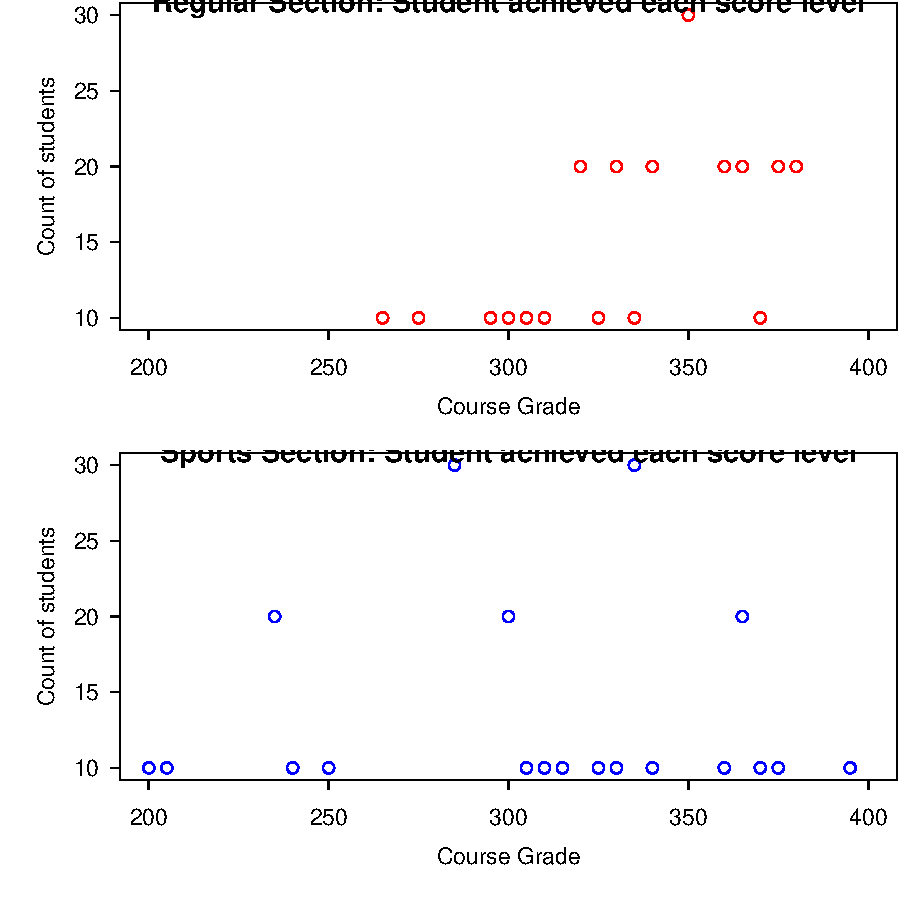
\includegraphics[width=.6\linewidth]{figure/DSC520-week-4-Testscore-TangXin-Rnwauto-report-1} 

}


\begin{kframe}\begin{alltt}
\hlstd{par_mfrow} \hlkwb{=} \hlkwd{c}\hlstd{(}\hlnum{1}\hlstd{,} \hlnum{1}\hlstd{)}
\end{alltt}
\end{kframe}
\end{knitrout}

The R session information (including the OS info, R version and all
packages used):

\begin{knitrout}
\definecolor{shadecolor}{rgb}{0.969, 0.969, 0.969}\color{fgcolor}\begin{kframe}
\begin{alltt}
\hlkwd{sessionInfo}\hlstd{()}
\end{alltt}
\begin{verbatim}
## R version 4.3.1 (2023-06-16 ucrt)
## Platform: x86_64-w64-mingw32/x64 (64-bit)
## Running under: Windows 10 x64 (build 19045)
## 
## Matrix products: default
## 
## 
## locale:
## [1] LC_COLLATE=English_United States.utf8  LC_CTYPE=English_United States.utf8   
## [3] LC_MONETARY=English_United States.utf8 LC_NUMERIC=C                          
## [5] LC_TIME=English_United States.utf8    
## 
## time zone: America/Chicago
## tzcode source: internal
## 
## attached base packages:
## [1] stats     graphics  grDevices utils     datasets  methods   base     
## 
## other attached packages:
## [1] readr_2.1.4   ggplot2_3.4.2 knitr_1.43    tinytex_0.45 
## 
## loaded via a namespace (and not attached):
##  [1] vctrs_0.6.2      cli_3.6.1        rlang_1.1.1      xfun_0.39        highr_0.10      
##  [6] generics_0.1.3   glue_1.6.2       colorspace_2.1-0 hms_1.1.3        scales_1.2.1    
## [11] fansi_1.0.4      grid_4.3.1       munsell_0.5.0    evaluate_0.21    tibble_3.2.1    
## [16] tzdb_0.4.0       lifecycle_1.0.3  compiler_4.3.1   dplyr_1.1.2      pkgconfig_2.0.3 
## [21] rstudioapi_0.14  R6_2.5.1         tidyselect_1.2.0 utf8_1.2.3       pillar_1.9.0    
## [26] magrittr_2.0.3   tools_4.3.1      withr_2.5.0      gtable_0.3.3
\end{verbatim}
\begin{alltt}
\hlkwd{Sys.time}\hlstd{()}
\end{alltt}
\begin{verbatim}
## [1] "2023-06-26 19:47:28 CDT"
\end{verbatim}
\end{kframe}
\end{knitrout}


\end{document}
